\documentclass{article}
\usepackage[main=spanish, provide=*]{babel}
\usepackage{xcolor}
\usepackage{sansmath}
\usepackage{array}
\usepackage{graphicx}
\usepackage{tikz}
\usepackage{circuitikz}
\usepackage{pgfplots}
\usepackage{darkmode}
\usepackage{amsmath}
\usepackage{svg}
\usepackage[a4paper, top=2cm, bottom=2cm]{geometry}

\sansmath
\renewcommand{\rmdefault}{cmss}

\newcommand{\iconpath}{/home/khz/git/tabler-icons/icons/outline-white/}
\newcommand{\icon}[1]{\includesvg[width=0.75em]{\iconpath#1}}
\newcommand{\instrumentopath}{/home/khz/Documentos/Carrera/MusiKe/instrumentos/svg/}
\newcommand{\instrumento}[1]{\raisebox{-0.6em}{\includesvg[width=2em]{\instrumentopath#1}}}

\enabledarkmode

\definecolor{c1}{HTML}{8bb6e7}
\definecolor{c2}{HTML}{87f3dd}
\definecolor{c3}{HTML}{fdef83}
\definecolor{c4}{HTML}{fdc373}
\definecolor{c5}{HTML}{fd8581}
\definecolor{c6}{HTML}{c573e7}
\definecolor{c7}{HTML}{afdb68}
\definecolor{c8}{HTML}{e59f8b}

\definecolor{page}{HTML}{262626}
\pagecolor{page}

\begin{document}
\title{MusiKe}
\author{Mario López Sáez}
\date{\today}
\maketitle

\begin{center}
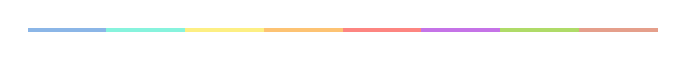
\begin{tikzpicture}
    \fill[c1] (0, 0) rectangle ++(1, 0.05);
    \fill[c2] (1, 0) rectangle ++(1, 0.05);
    \fill[c3] (2, 0) rectangle ++(1, 0.05);
    \fill[c4] (3, 0) rectangle ++(1, 0.05);
    \fill[c5] (4, 0) rectangle ++(1, 0.05);
    \fill[c6] (5, 0) rectangle ++(1, 0.05);
    \fill[c7] (6, 0) rectangle ++(1, 0.05);
    \fill[c8] (7, 0) rectangle ++(1, 0.05);
\end{tikzpicture}

\end{center}

\tableofcontents
\newpage



\section{Descripción del Proyecto}

MusiKe es un juego educativo e interactivo diseñado para que usuarios de todas las edades descubran y aprendan los instrumentos de la orquesta a través de divertidos retos y minijuegos. La aplicación está desarrollada para Android usando Java y la librería AppCompat.

\section{Estructura del Proyecto}

\begin{itemize}
  \item \icon{folder} \textbf{app/src/main/java/mario/khz/musike}: contiene las actividades y clases principales de la aplicación.
  \item \icon{photo-scan} \textbf{app/src/main/res/drawable}: recursos gráficos vectoriales (iconos de instrumentos, fondos y botones).
  \item \icon{volume-2} \textbf{app/src/main/res/raw}: archivos de audio con sonidos de los instrumentos de la orquesta.
  \item \icon{file-text} \textbf{README.md}: descripción general del proyecto y logo.
  \item \icon{file} \textbf{tex/MusiKe.tex}: este documento de documentación.
\end{itemize}

\newpage

\section{Assets}

\subsection{Instrumentos \icon{music}}

A continuación se listan los instrumentos incluidos en la aplicación, junto a sus recursos gráficos y de audio:

\begin{itemize}
  \item \instrumento{viola} Violín: \texttt{res/drawable/violin.xml}, \texttt{res/raw/violin.mp3}
  \item \instrumento{viola} Viola: \texttt{res/drawable/viola.xml}, \texttt{res/raw/viola.mp3}
  \item \instrumento{cello} Violonchelo: \texttt{res/drawable/cello.xml}, \texttt{res/raw/cello.mp3}
  \item \instrumento{contrabajo} Contrabajo: \texttt{res/drawable/contrabajo.xml}, \texttt{res/raw/contrabajo.mp3}
  \item \instrumento{piano} Piano: \texttt{res/drawable/piano.xml}, \texttt{res/raw/piano.mp3}
  \item \instrumento{flauta} Flauta: \texttt{res/drawable/flauta.xml}, \texttt{res/raw/flauta.mp3}
  \item \instrumento{oboe} Oboe: \texttt{res/drawable/oboe.xml}, \texttt{res/raw/oboe.mp3}
  \item \instrumento{clarinete} Clarinete: \texttt{res/drawable/clarinete.xml}, \texttt{res/raw/clarinete.mp3}
  \item \instrumento{fagot} Fagot: \texttt{res/drawable/fagot.xml}, \texttt{res/raw/fagot.mp3}
  \item \instrumento{trompeta} Trompeta: \texttt{res/drawable/trompeta.xml}, \texttt{res/raw/trompeta.mp3}
  \item \instrumento{trombon} Trombón: \texttt{res/drawable/trombon.xml}, \texttt{res/raw/trombon.mp3}
  \item \instrumento{trompa} Trompa: \texttt{res/drawable/trompa.xml}, \texttt{res/raw/trompa.mp3}
  \item \instrumento{tuba} Tuba: \texttt{res/drawable/tuba.xml}, \texttt{res/raw/tuba.mp3}
  \item \instrumento{arpa} Arpa: \texttt{res/drawable/arpa.xml}, \texttt{res/raw/arpa.mp3}
  \item \instrumento{marimba} Marimba: \texttt{res/drawable/marimba.xml}, \texttt{res/raw/marimba.mp3}
  \item \instrumento{vibrafono} Vibráfono: \texttt{res/drawable/vibrafono.xml}, \texttt{res/raw/vibrafono.mp3}
  \item \instrumento{pequena_percusion} Pequeña percusión: \texttt{res/drawable/pequena\_percusion.xml}, \texttt{res/raw/pequena\_percusion.mp3}
  \item \instrumento{platos_de_choque} Platos de choque: \texttt{res/drawable/platos\_de\_choque.xml}, \texttt{res/raw/platos\_de\_choque.mp3}
  \item \instrumento{campanologo} Campanólogo: \texttt{res/drawable/campanologo.xml}, \texttt{res/raw/campanologo.mp3}
  \item \instrumento{caja} Caja: \texttt{res/drawable/caja.xml}, \texttt{res/raw/caja.mp3}
\end{itemize}
\newpage
\subsection{Iconos de Instrumentos}

Los iconos de los instrumentos han sido obtenidos de \texttt{https://www.freepik.com/} y procesados posteriormente con el siguiente código:

\begin{figure}[h]
\centering
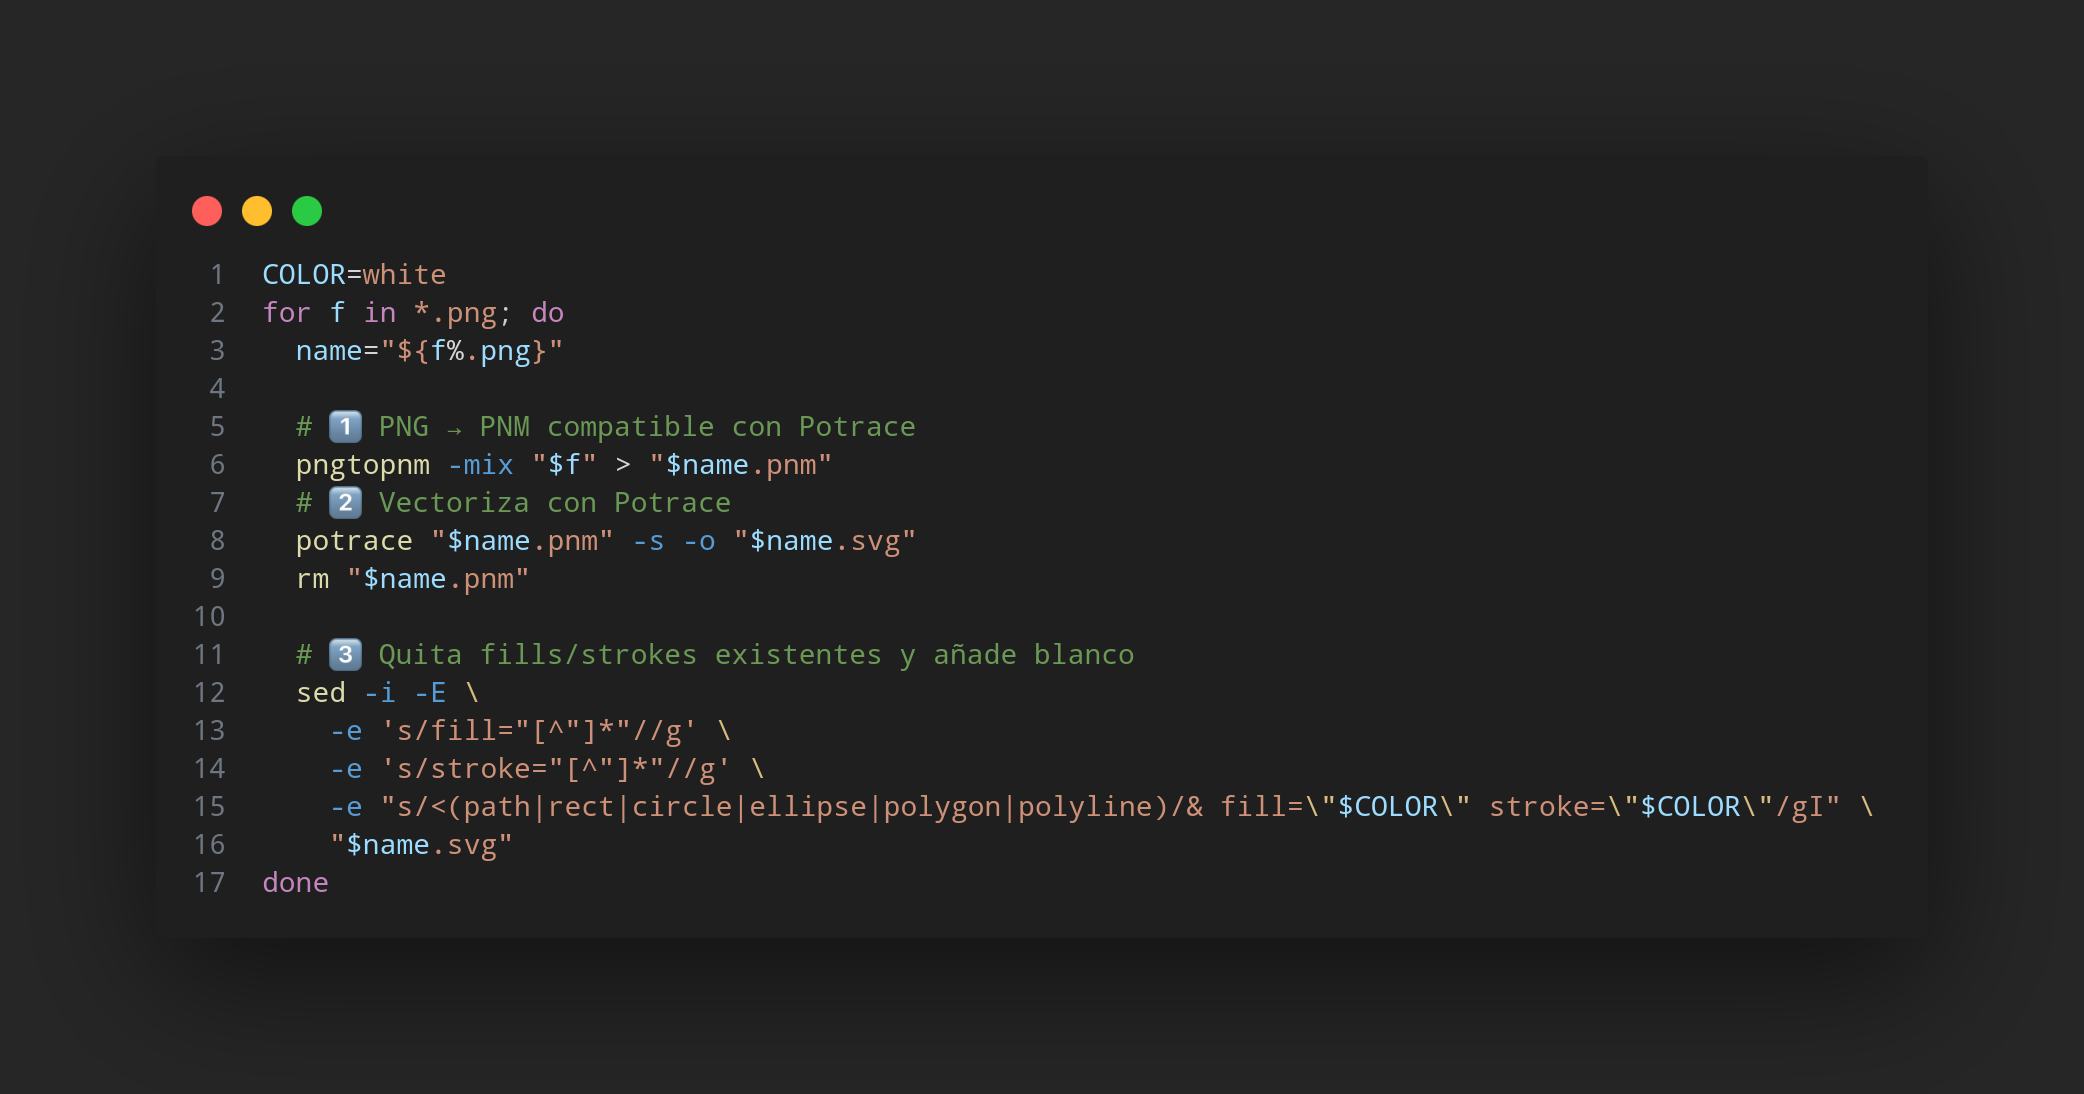
\includegraphics[width=\textwidth]{svg_codigo.png}
\caption{Código de procesamiento de SVG.}
\end{figure}


\section{Activities}

La arquitectura de la aplicación se articula en torno a un conjunto de Activities, cada una responsable de una pantalla y una funcionalidad concreta. A continuación, se detalla el propósito y funcionamiento de cada una de ellas.

\subsection{MainActivity \icon{layout-dashboard}}
Es la actividad principal y el punto de entrada de la aplicación. Su función es presentar al usuario la pantalla de bienvenida y actuar como un distribuidor central, ofreciendo las dos modalidades principales de la aplicación:
\begin{itemize}
    \item \textbf{Modo Estudio}: Inicia \texttt{StudyActivity} para el aprendizaje libre.
    \item \textbf{Modo Juego}: Lanza \texttt{RoundSelectionActivity} para comenzar una partida.
\end{itemize}

\subsection{StudyActivity \icon{book}}
Esta actividad está diseñada para el aprendizaje y la consulta. Proporciona una interfaz donde el usuario puede explorar todos los instrumentos de la orquesta. Al seleccionar un instrumento, la actividad reproduce su sonido característico, permitiendo una familiarización auditiva y visual sin la presión de un entorno de juego.

\subsection{RoundSelectionActivity \icon{list}}
Actúa como una antesala al modo de juego. Su único propósito es permitir al usuario configurar la partida, seleccionando el número de rondas que desea jugar. Una vez que el usuario ha hecho su elección, esta actividad inicia la \texttt{GameActivity}, pasándole la configuración seleccionada como un \textit{extra} en el \texttt{Intent}.

\subsection{GameActivity \icon{device-gamepad-2}}
Es el núcleo interactivo de MusiKe. Esta actividad gestiona la lógica del juego de identificación de instrumentos, que se desarrolla de la siguiente manera:
\begin{itemize}
    \item \textbf{Inicio y carga}: Al comenzar, lee el fichero \texttt{assets/instruments.json} para cargar la información de los instrumentos. A continuación, baraja la lista para crear un orden aleatorio de preguntas para la partida.
    \item \textbf{Desarrollo de la ronda}: En cada ronda, reproduce el sonido de un instrumento y presenta al usuario cuatro botones con nombres de instrumentos como posibles respuestas. Para aumentar el desafío, las opciones incorrectas se eligen preferentemente de la misma familia que la respuesta correcta.
    \item \textbf{Interacción y feedback}: El usuario selecciona una opción. La aplicación le proporciona feedback visual inmediato (verde para acierto, rojo para error) y sonoro. Si falla, se le indica cuál era la respuesta correcta. Tras una breve pausa, la actividad avanza automáticamente a la siguiente ronda.
    \item \textbf{Finalización}: Una vez completadas todas las rondas, \texttt{GameActivity} recopila las estadísticas de la partida (número de aciertos, respuestas del usuario y respuestas correctas) y lanza la \texttt{FinishActivity} para mostrar los resultados.
\end{itemize}

\subsection{FinishActivity \icon{award}}
Esta es la pantalla final del ciclo de juego. Su objetivo es mostrar al usuario un resumen de su rendimiento en la partida. Presenta la puntuación final (ej: "8 de 10 aciertos") y una tabla detallada que muestra las respuestas correctas para cada ronda, reforzando así el aprendizaje.

\subsection{CircleProgressView \icon{chart-pie}}
Aunque no es una Activity, es un componente de interfaz de usuario (View) personalizado de vital importancia en \texttt{GameActivity}. Su función es mostrar una barra de progreso circular que se actualiza en tiempo real, sincronizada con la reproducción del audio del instrumento. Esto proporciona al usuario una referencia visual clara de la duración del sonido y del tiempo restante para responder, mejorando significativamente la experiencia de juego.

\end{document}
